Now that the requirements necessary to build the system have been formulated, potential solutions to fulfil the list of requirements from Chapter \ref{ch:chapter3} for each aspect of the system can now be analysed before a final solution can be chosen. The first section of this chapter will focus on different solutions for the system's pipeline, starting with the offline feature extraction phase, followed by the online retrieval phase, and ending with the database pre-processing phase. The second section will focus on general design decisions such as the programming language, the type of interface and the type of videos to use. These two sections will be used to outline the final chosen solutions for each aspect of the system before a development plan can be devised.

\section{Pipeline Design Analysis}

Explore possible options for different sections of the system, such as:
    \begin{itemize}
        \item types of features to extract (why static colour features and not object/motion features) - histograms are very popular with videos, calculations are easier, implementation is easier, results are as efficient
        \item types of learning models (histogram matching, BoW-approach VS Neural Network)
    \end{itemize}
    
\begin{figure}[h]
\centerline{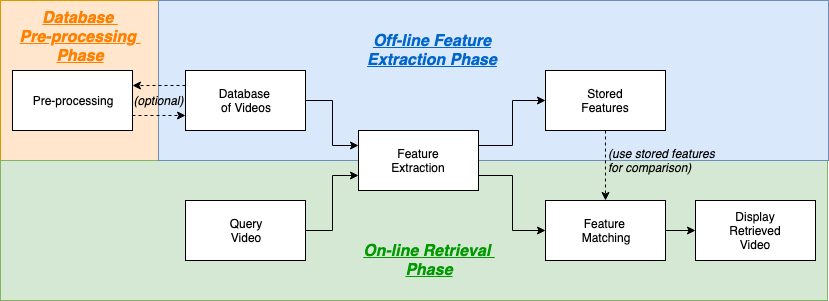
\includegraphics[width=1.15\textwidth]{figures/design/basic_cbvr_phases.png}}
\caption{\label{fig:basic-cbvr-diagram}Basic CBVR system diagram.}
\end{figure}

\subsection{Offline Feature Extraction Phase}

todo

\subsection{Online Retrieval Phase}

todo

\subsection{Database Pre-Processing Phase}

todo

\section{General Project Design}

decision on programming language, on database videos and interface choice

\subsection{Programming Language}

\begin{itemize}
	\item python VS MATLAB vs other languages
	\item rich array of libraries: OpenCV, NumPy, SciPy, MatplotLib
	\item ease of installing third-party libraries with PIP
	\item powerful IDEs (PyCharm)
	\item ease of generating testing suites
     \item familiarity with
\end{itemize}

\subsection{Interface}

interface choice (why CLI VS GUI?): time constraints and no users, goal of this project is to research efficient results, not create a commercial product

\subsection{Database videos}

types of videos in databases (why short videos VS movies, cartoons/stop-motion pictures)

\section{Chosen Solution}

include a high-level diagram of system excluding detail (all DB videos in system, single query video in system, matching video output)

\section{Development Plan}

plan with time constraints in mind

\section{Summary}

summarise section
